\begin{figure}[!htb]
	\centering

	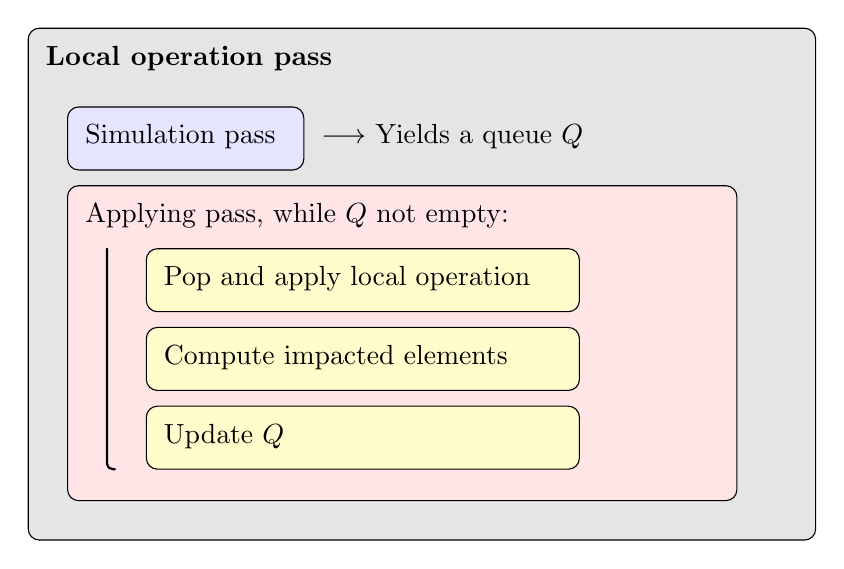
\begin{tikzpicture}

		\draw[rounded corners, fill=black!10] (0, 0) rectangle (10, 6.5);
		\node[anchor=north west,font=\bfseries, xshift=0.1cm, yshift=-0.1cm] at (0,6.5) {Local operation pass};

		\draw[rounded corners, fill=blue!10] (0.5, 4.7) rectangle (3.5, 5.5);
		\node[anchor=north west, xshift=0.1cm, yshift=-0.1cm] at (0.5,5.5) {Simulation pass};

		\node[anchor=north west, xshift=0.1cm, yshift=-0.1cm] at (3.5,5.5) {$\longrightarrow$ Yields a queue
			$Q$};

		\draw[rounded corners, fill=red!10] (0.5, 0.5) rectangle (9, 4.5);
		\node[anchor=north west, xshift=0.1cm, yshift=-0.1cm] at (0.5,4.5) {Applying pass, while $Q$ not empty:};

		\draw[thick, rounded corners=2pt, line cap = round, line join = round] (1,3.7) -- (1,0.9) -- (1.1,0.9);

		\draw[rounded corners, fill=yellow!20] (1.5, 2.9) rectangle (7, 3.7);
		\node[anchor=north west, xshift=0.1cm, yshift=-0.1cm] at (1.5,3.7) {Pop and apply local operation};

		\draw[rounded corners, fill=yellow!20] (1.5, 1.9) rectangle (7, 2.7);
		\node[anchor=north west, xshift=0.1cm, yshift=-0.1cm] at (1.5,2.7) {Compute impacted elements};

		\draw[rounded corners, fill=yellow!20] (1.5, 0.9) rectangle (7, 1.7);
		\node[anchor=north west, xshift=0.1cm, yshift=-0.1cm] at (1.5,1.7) {Update $Q$};

	\end{tikzpicture}

	\caption{Local operation scheme}\label{fig:localOperationPass}
\end{figure}
